\section{Technical validation of the reported study}
\label{app:technical_validation}

\subsection{Frozen detector, training record, and scoring contract}

All primary detector-response analyses use the same EfficientNetV2-S checkpoint:
training seed 42, epoch 160, SHA-256
\texttt{5d1082839aac7a0b\allowbreak
fb89342f84a9a533\allowbreak
b22e1111c15cb471\allowbreak
1255ed1b524a2b8d}. Section~\ref{sec:detector_training} defines the primary
training and checkpoint rules; Section~\ref{sec:checkpoint_panel_design}
separately defines the 12-run sensitivity panel. The archived training
configuration and checkpoint hash identify the exact primary model.

The retained checkpoint-validation summary contains 61,437 negatives and 778
noisy catalogue-positive labels. At native-logit precision its ROC AUC is
0.96531. Average precision is 0.79659 from native logits and 0.79173 from
float32 sigmoid scores because 287 probabilities saturate at one; the
float64-probability Brier score is 0.005169. These values describe the
recorded noisy-label validation set. The operating threshold and
selected-system evaluation use their dedicated cohorts.

Applying Equation~\ref{eq:common_threshold} to the 20,002 calibration rows
gives \(t=1.5717214345932007\) (float32 bits 1070149163), with 20
exceedances and comparator \(\ell\geq t\). Scoring uses the checkpoint above
in evaluation mode, a fixed batch width of 64, native float32 logits, stored
batch-normalisation statistics, inactive dropout, and an MPS
(\emph{Metal Performance Shaders}) backend whose software and hardware
profile is checksum-bound. Padding repeats the final real row; filler outputs
are discarded. The bitwise checks apply to this MPS backend and batch
configuration; other hardware or software environments may produce small
numerical differences.

The separate achieved-FPR endpoint contains 12,512 catalogue-negative rows
in 1,089 spatial groups and was not used to recalibrate \(t\). It has 13
exceedances, or 0.001039. The row-Wilson interval is
[0.000607, 0.001777], and the spatial-group multiplier interval is
[0.000546, 0.001656]. A separate author-run implementation checks the
manifest and 12,512 payload arrays and reproduces the native score bits,
threshold decisions, and result calculation.

\begin{table*}
\caption{Full-precision primary results underlying the rounded main-text
values. Intervals are the procedures defined in Section~\ref{sec:analysis_design};
movements are fold-standardised units and effects are percentage points.}
\label{tab:primary_full_precision}
\centering
\begin{tabular}{lll}
\toprule
Quantity & Estimate & Interval or diagnostic \\
\midrule
Threshold & 1.5717214345932007 & float32 bits 1070149163 \\
Achieved FPR & 13/12\,512 = 0.103900\% &
spatial-group 0.054580--0.165564\% \\
Selected systems & 39/43 = 90.697674\% & finite cohort \\
\(G_{\rm rec}\) & 3.454545\% & 3.097551--3.830632\% \\
\(G_{\rm domain}\) AUC &
0.991340 / 0.958187 / 0.978528 / 0.980745 &
operational / Stein / ImageNet / pixel \\
Fixed-head domain ranking & 0.980306 & existing operational lens logit \\
\(G_{\rm match}\) movement &
+0.023183 / +0.235027 / +0.024792 / -0.029207 &
operational / Stein / ImageNet / pixel \\
\(P_{\rm noise}\) & -1.203030 & [-1.387747, -1.027768]; MCSE 0.013886 \\
\(P_{\rm src}\) & +0.560290 & [+0.283912, +0.932231]; MCSE 0.042076 \\
\bottomrule
\end{tabular}
\end{table*}

\subsection{Four-representation probe diagnostics}
\label{app:four_representation_diagnostics}

The operational feature extraction uses the primary checkpoint's
1,280-component pooled penultimate output. The final \(G_{\rm domain}\)
feature matrices contain 6,379 rows, and the final domain and matched
manifests together contain 6,444 unique pixel payloads. On the recorded MPS
backend, applying the retained linear classifier to the final operational
features reconstructs all 6,379 native logits bit for bit. Separate
same-version refits from each of the four persisted final domain matrices
reproduce every OOF score exactly. These checks verify the archived arrays and
estimator implementation; they are not independent scientific replications.

Table~\ref{tab:gdomain_fold_diagnostics} gives the five fold diagnostics.
Each fold contains only 8 or 9 observed systems. The pooled OOF AUC is the
prespecified finite-cohort summary; the fold values show the support and
variation across its five fitted readouts.

\begin{table*}
\caption{\(G_{\rm domain}\) weighted OOF AUC by frozen dependency fold.
Observed support is 8, 9, 8, 9, and 9 systems in folds 0--4; simulated support
is 1,276, 1,265, 1,265, 1,265, and 1,265 rows.}
\label{tab:gdomain_fold_diagnostics}
\centering
\begin{tabular}{lrrrrr}
\toprule
Feature protocol & Fold 0 & Fold 1 & Fold 2 & Fold 3 & Fold 4 \\
\midrule
Operational penultimate & 0.985194 & 0.996212 & 0.992515 & 0.994124 & 0.999320 \\
Stein SSL & 0.952142 & 0.974942 & 0.999945 & 0.976933 & 0.929293 \\
Generic ImageNet & 0.969132 & 0.953089 & 0.993990 & 0.978681 & 0.992036 \\
Pixel statistics & 0.937664 & 0.996503 & 0.993990 & 0.974699 & 0.986694 \\
\bottomrule
\end{tabular}
\end{table*}

The fixed operational head uses the same component/class weights but no
domain-probe fit. Its component-weighted AUC is 0.9803064184, compared with
row-weighted AUC 0.9812331160. Median native logits are 19.6848 for observed
references and \(-22.6331\) for injections. These are selected-population
descriptives, not calibrated probabilities.

\begin{table*}
\caption{Native operational-logit distribution on the exact
\(G_{\rm domain}\) populations. Entries are finite-cohort quantiles.}
\label{tab:fixed_head_logit_quantiles}
\centering
\begin{tabular}{lrrrrr}
\toprule
Population & 5\% & 25\% & 50\% & 75\% & 95\% \\
\midrule
Observed & -1.70 & 13.58 & 19.68 & 23.54 & 26.08 \\
Injected & -27.07 & -24.32 & -22.63 & -19.73 & 0.20 \\
\bottomrule
\end{tabular}
\end{table*}

\subsection{Conditional PSF--depth--radius response}
\label{app:cell_radius_response}

All 99 occupied cell--radius summaries were reproduced directly from the final
49,500 score rows. Each entry contains 500 distinct targets. The design has
five PSF nodes and two depth nodes but occupies nine of the ten possible
combinations; PSF 1.05 arcsec at depth 24.0 mag is empty. Figure
\ref{fig:cell_radius_response} shows the occupied support rather than
interpolating the missing cell.

\begin{figure*}
\centering
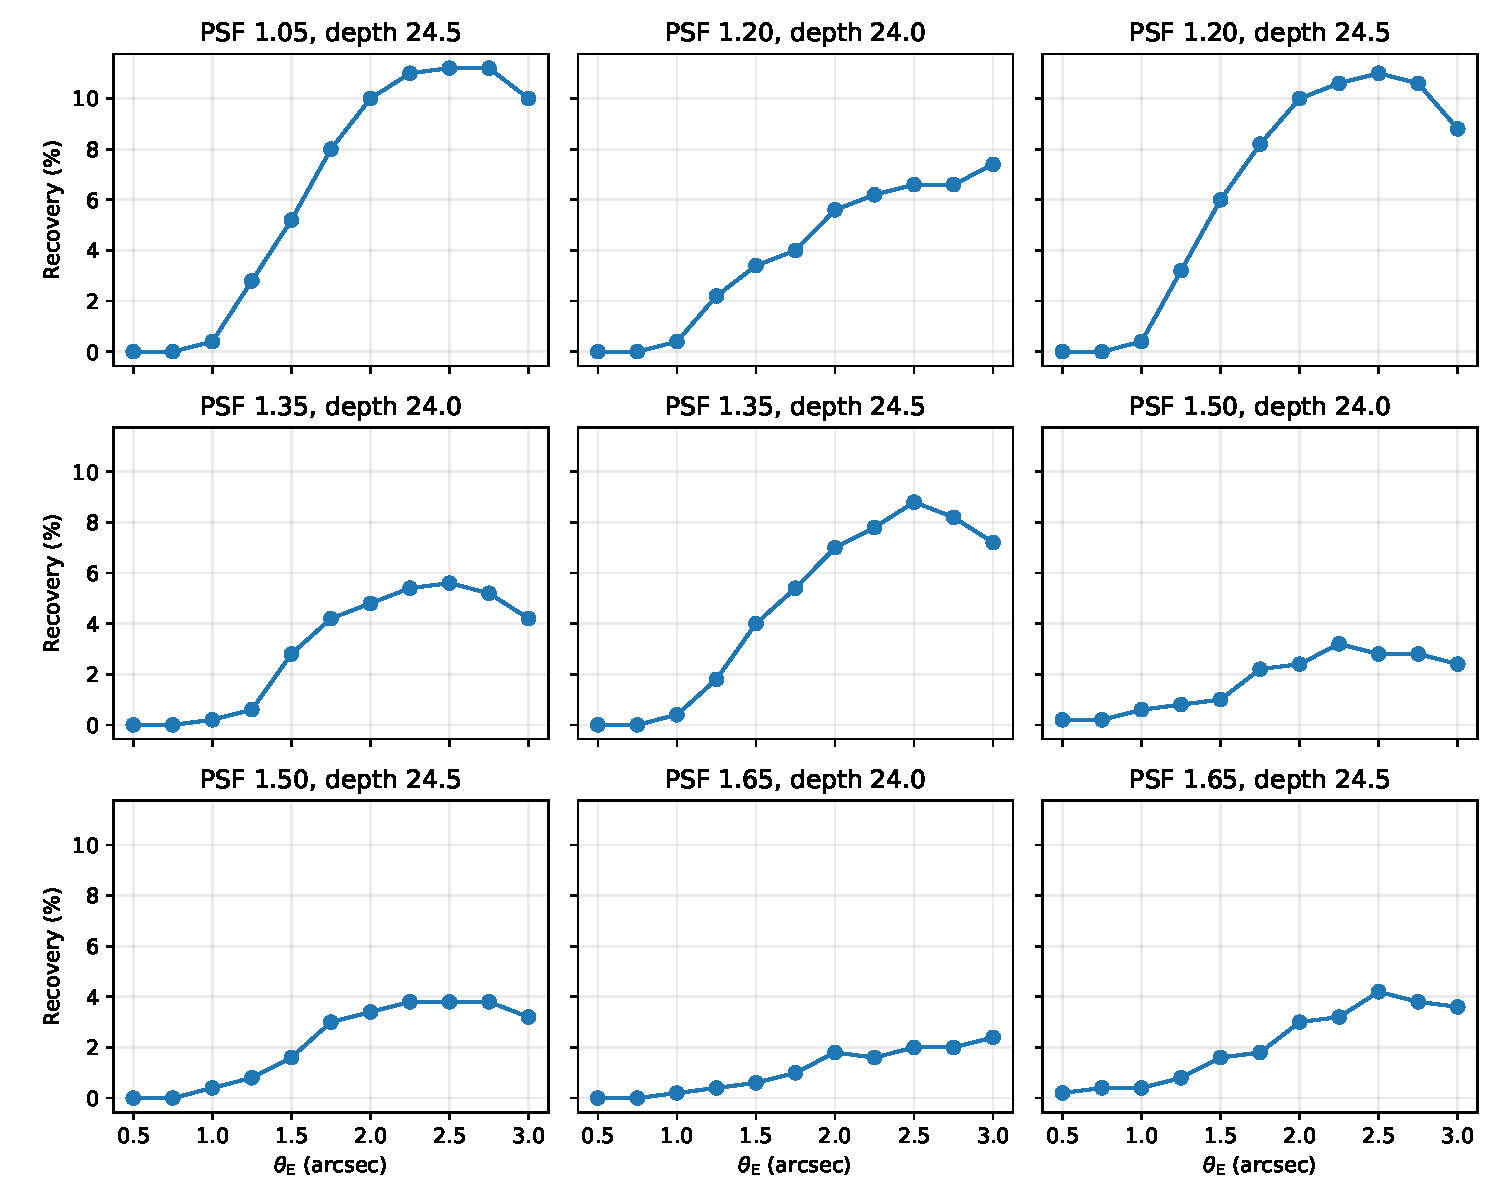
\includegraphics[width=\textwidth]{figures/appendix_grec_cell_radius_response.pdf}
\caption{Conditional \(G_{\rm rec}\) recovery versus Einstein radius in each
occupied PSF--depth cell. Every point contains 500 targets. The panels are
descriptive support strata covering nine of the ten possible PSF--depth
combinations.}
\label{fig:cell_radius_response}
\par\smallskip{\raggedright\noindent\textit{Alt text:} Nine panels show
recovery curves over eleven Einstein radii for the occupied combinations of
five PSF values and two depth values. The PSF 1.05, depth 24.0 combination is
absent from the design.\par}
\end{figure*}

\subsection{Fixed-target brightness and source-photon response}
\label{app:bounded_controls}

The brightness control contains 344 target--magnitude cells, 344 expectation
images, and 2,752 photon realizations. Table~\ref{tab:brightness_control}
reports equal-target recovery; photon rates first average eight draws within
target. Eight-draw finite-photon MCSE is at most 1.071 percentage points. Zero MCSE at
the faint nodes reflects eight all-negative draw-specific cohort rates, not a
general precision guarantee.

\begin{figure*}
\refstepcounter{table}\label{tab:brightness_control}
\noindent\textbf{Table~\thetable.} Fixed-target \(C_{\rm bright}\) recovery
percentages under the trained preprocessing and common threshold.
\begin{center}
\begin{tabular}{rrr}
\toprule
\(m_{r,\mathrm{src}}\) & Expectation & Photon \\
\midrule
18.5 & 13.953 & 12.500 \\
19.5 & 16.279 & 13.081 \\
20.5 & 18.605 & 18.314 \\
21.5 & 11.628 & 13.953 \\
22.5 & 9.302 & 7.558 \\
23.5 & 2.326 & 1.744 \\
24.5 & 0.000 & 0.000 \\
25.5 & 0.000 & 0.000 \\
\bottomrule
\end{tabular}
\end{center}
\medskip
\centering
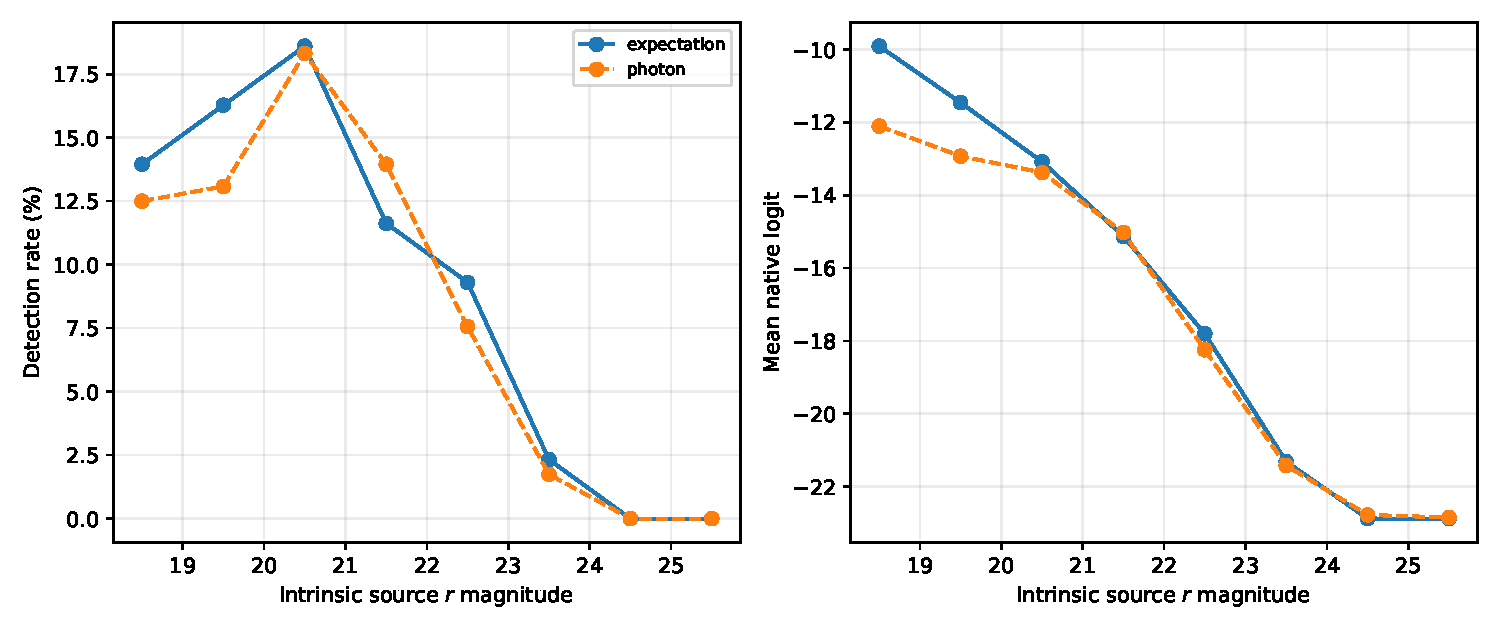
\includegraphics[width=0.9\textwidth]{figures/appendix_brightness_response.pdf}
\caption{Detection fraction and mean native logit versus intrinsic source
magnitude for the fixed 43-target brightness experiment. Expectation and
photon-realized images use the trained preprocessing and common threshold.
The detection fraction peaks near magnitude 20.5, whereas the mean logit
declines across the tested magnitude range. These are finite-cohort response
summaries on 43 fixed targets.}
\label{fig:brightness_response}
\par\smallskip{\raggedright\noindent\textit{Alt text:} Two panels show
expectation and photon-realized images over intrinsic source magnitudes 18.5
to 25.5. Detection fractions reach their maximum at 20.5 and are zero at 24.5
and 25.5. Mean logits decline toward fainter magnitudes. The photon and
expectation curves are close but not identical.\par}
\end{figure*}

This finite-cohort detector-response test characterizes the fixed targets and
tested source scalings; intrinsic magnitude supplies the controlled axis.
\FloatBarrier
\clearpage

\subsection{\(P_{\rm noise}\) draw-count pilot}
\label{app:pnoise_draw_pilot}

\noindent\begin{minipage}{\columnwidth}
The score-blind pilot contains 288 targets and 3,168 scenes, with 64 draws per
scene. MCSE and the target-sampling standard error are on the probability scale;
the latter is 0.003553. A candidate passes when MCSE is at most 0.002 and at
most 20 per cent of the target-sampling standard error. One draw is diagnostic
only because its MCSE is unavailable; eight is the smallest count satisfying
both criteria.

\begin{center}
\refstepcounter{table}\label{tab:pnoise_draw_pilot}
\noindent\textbf{Table~\thetable.} \(P_{\rm noise}\) design-pilot
photon-draw selection.
\par\smallskip
\scriptsize
\begin{tabular}{rcccc}
\toprule
Draws & MCSE & MCSE/SE & Absolute criterion & Relative criterion \\
\midrule
1  & unavailable & unavailable & No & No \\
2  & 0.001119 & 0.315 & Yes & No \\
4  & 0.000791 & 0.223 & Yes & No \\
\textbf{8}  & \textbf{0.000559} & \textbf{0.157} & \textbf{Yes} & \textbf{Yes} \\
16 & 0.000396 & 0.111 & Yes & Yes \\
32 & 0.000280 & 0.079 & Yes & Yes \\
64 & 0.000198 & 0.056 & Yes & Yes \\
\bottomrule
\end{tabular}
\end{center}
\end{minipage}

\subsection{Detector-checkpoint sensitivity}
\label{app:checkpoint_sensitivity}

Tables~\ref{tab:checkpoint_panel_endpoints} and
\ref{tab:checkpoint_panel_interventions} report the runs defined in
Section~\ref{sec:checkpoint_panel_design}, selected and calibrated as in
Section~\ref{sec:checkpoint_sensitivity_methods}. The within-run selection
metric is average precision from float32 sigmoid outputs on that run's
noisy-label validation population; an exact tie retains the earliest epoch.
The primary detector remains the terminal epoch-160 checkpoint.

\begin{table*}
\refstepcounter{table}\label{tab:checkpoint_panel_endpoints}
\noindent\textbf{Table~\thetable.} Final checkpoint-sensitivity endpoints.
Each \(t_m\) yields exactly 20 threshold exceedances among the same 20,002
calibration negatives. Achieved-FPR counts use the same 12,512-row evaluation
cohort; their percentages and the \(G_{\rm rec}\) percentages are followed by
95 per cent spatial-group intervals. Selected-system entries are exact counts
among the same 43 systems. Baseline denotes natural-prevalence sampling with
cosine scheduling; the other variant labels name the one changed training
factor. ``Both sources'' uses reviewed and additional catalogue candidates;
``Reviewed only'' omits the additional candidates. Validation AP is the
within-run checkpoint-selection value; values for the two positive-example
compositions are computed on validation populations with 778 and 64 noisy
positive labels, respectively, and should not be compared as if their labels
or prevalence were the same. The target FPR is an empirical calibration rate
rather than a guaranteed population rate.
\begin{center}
\scriptsize
\begin{tabular}{L{0.09\textwidth}L{0.07\textwidth}r r r r
                L{0.205\textwidth}r L{0.20\textwidth}}
\toprule
Variant & Positive examples & Seed & Epoch & Val.\ AP & \(t_m\) &
Achieved FPR: count; per cent [interval] & Selected &
\(G_{\rm rec}\): per cent [interval] \\
\midrule
Baseline & Both sources & 42 & 19 & 0.8104 & 1.153126 &
11; 0.0879 [0.0434, 0.1454] & 35/43 & 2.5717 [2.2801, 2.8757] \\
Baseline & Both sources & 123 & 17 & 0.8181 & 0.621170 &
13; 0.1039 [0.0550, 0.1656] & 37/43 & 2.4263 [2.1344, 2.7286] \\
Baseline & Both sources & 2026 & 93 & 0.8053 & 3.659930 &
16; 0.1279 [0.0738, 0.1948] & 37/43 & 3.1535 [2.8163, 3.5084] \\
\addlinespace
Baseline & Reviewed only & 42 & 103 & 0.7764 & -9.486459 &
17; 0.1359 [0.0773, 0.2093] & 37/43 & 1.8485 [1.6015, 2.1177] \\
Baseline & Reviewed only & 123 & 93 & 0.7704 & -8.606620 &
21; 0.1678 [0.1047, 0.2454] & 36/43 & 1.4525 [1.2305, 1.6973] \\
Baseline & Reviewed only & 2026 & 43 & 0.7679 & -1.618260 &
16; 0.1279 [0.0700, 0.2059] & 36/43 & 1.2808 [1.0801, 1.4987] \\
\addlinespace
50:50 sampler & Both sources & 42 & 62 & 0.7922 & 6.281433 &
12; 0.0959 [0.0502, 0.1552] & 35/43 & 2.8081 [2.4995, 3.1276] \\
50:50 sampler & Reviewed only & 42 & 37 & 0.7704 & -7.143696 &
17; 0.1359 [0.0751, 0.2150] & 37/43 & 1.3778 [1.1665, 1.6091] \\
\addlinespace
Step schedule & Both sources & 42 & 18 & 0.8109 & 1.875446 &
9; 0.0719 [0.0333, 0.1255] & 35/43 & 2.1071 [1.8303, 2.3978] \\
Step schedule & Reviewed only & 42 & 87 & 0.7653 & -2.322129 &
14; 0.1119 [0.0620, 0.1777] & 35/43 & 1.3636 [1.1628, 1.5833] \\
\addlinespace
Additional seed & Reviewed only & 7 & 86 & 0.7516 & -7.043954 &
14; 0.1119 [0.0611, 0.1763] & 39/43 & 1.3980 [1.1897, 1.6259] \\
Additional seed & Reviewed only & 2027 & 99 & 0.7695 & -9.008804 &
19; 0.1519 [0.0872, 0.2345] & 36/43 & 1.4040 [1.1922, 1.6399] \\
\bottomrule
\end{tabular}
\end{center}
\end{table*}

\medskip
\begin{table*}
\refstepcounter{table}\label{tab:checkpoint_panel_interventions}
\noindent\textbf{Table~\thetable.} Final checkpoint sensitivity of the paired
interventions. \(P_{\rm noise}\) is
modelled-photon-minus-expectation and
\(P_{\rm src}\) is S\'{e}rsic-minus-structured. Every row uses its
checkpoint-specific threshold yielding exactly 20 exceedances among 20,002
calibration negatives.
Estimates, intervals, and MCSE values are percentage points. The 95 per cent
intervals use one global target-spatial-group multiplier for
\(P_{\rm noise}\). For \(P_{\rm src}\), each pair receives the product of
global target-spatial and source multipliers, with source multipliers
normalised within the 16 source strata. MCSE uses the eight photon draws.
Baseline denotes natural-prevalence sampling with cosine scheduling; the
other variant labels name the one changed training factor. ``Both sources''
uses reviewed and additional catalogue candidates; ``Reviewed only'' omits
the additional candidates.
Intervals condition on the displayed checkpoint-specific thresholds and omit
calibration-sample variation.
\begin{center}
\scriptsize
\begin{tabular}{L{0.095\textwidth}L{0.075\textwidth}r r
                L{0.23\textwidth}r L{0.23\textwidth}r}
\toprule
Variant & Positive examples & Seed & Epoch &
\(P_{\rm noise}\) [95\% interval] & MCSE &
\(P_{\rm src}\) [95\% interval] & MCSE \\
\midrule
Baseline & Both sources & 42 & 19 & -0.9679 [-1.1321, -0.8137] & 0.0122 &
+0.3946 [+0.1622, +0.7152] & 0.0569 \\
Baseline & Both sources & 123 & 17 & -0.8379 [-0.9854, -0.7017] & 0.0120 &
+0.2683 [+0.0278, +0.5723] & 0.0207 \\
Baseline & Both sources & 2026 & 93 & -1.1644 [-1.3399, -0.9983] & 0.0130 &
+0.4261 [+0.1349, +0.8361] & 0.0651 \\
\addlinespace
Baseline & Reviewed only & 42 & 103 & -0.9672 [-1.1183, -0.8282] & 0.0088 &
+0.1184 [-0.0456, +0.3366] & 0.0303 \\
Baseline & Reviewed only & 123 & 93 & -0.7341 [-0.8719, -0.6123] & 0.0073 &
+0.0947 [-0.0411, +0.2952] & 0.0442 \\
Baseline & Reviewed only & 2026 & 43 & -0.7813 [-0.9180, -0.6529] & 0.0067 &
+0.0710 [-0.1679, +0.3166] & 0.0251 \\
\addlinespace
50:50 sampler & Both sources & 42 & 62 & -0.9982 [-1.1705, -0.8406] & 0.0129 &
+0.3946 [+0.1512, +0.7127] & 0.0752 \\
50:50 sampler & Reviewed only & 42 & 37 & -0.5111 [-0.6272, -0.4054] & 0.0091 &
+0.2446 [+0.0809, +0.5178] & 0.0469 \\
\addlinespace
Step schedule & Both sources & 42 & 18 & -0.7162 [-0.8697, -0.5764] & 0.0114 &
+0.3157 [+0.1297, +0.6001] & 0.0506 \\
Step schedule & Reviewed only & 42 & 87 & -0.8048 [-0.9429, -0.6789] & 0.0072 &
+0.1736 [+0.0530, +0.4061] & 0.0231 \\
\addlinespace
Additional seed & Reviewed only & 7 & 86 & -0.8535 [-1.0025, -0.7184] & 0.0073 &
+0.0947 [-0.0406, +0.2676] & 0.0207 \\
Additional seed & Reviewed only & 2027 & 99 & -0.7856 [-0.9292, -0.6546] & 0.0077 &
+0.0947 [-0.0740, +0.2794] & 0.0267 \\
\bottomrule
\end{tabular}
\end{center}
\end{table*}

The two-policy comparison, including designation of the validation-selected
policy for the main presentation, is exploratory. Under both policies all
12 aggregate \(P_{\rm noise}\) estimates are negative with intervals below
zero, and all 12 \(P_{\rm src}\) estimates are positive. Source-effect
intervals exclude zero for 7/12 validation-selected checkpoints and 8/12
terminal-epoch checkpoints. These related analyses describe policy
sensitivity within the same training runs.

A separate author-run
verification implementation reproduces the validation-selected epochs,
recorded checkpoint hashes, thresholds, row identities, estimates, intervals,
and MCSE values.

\subsection{Descriptive attribution of the pixel-statistic probe}

Using the same dependency-closed folds, component weights, and fold-local
standardisation, a secondary descriptive suite refits each of the 18
statistics alone and after its omission, and likewise evaluates each
photometric band. Median \(z\)-band pixel intensity is strongest: its
univariate OOF AUC is 0.888, omitting it reduces the multivariate AUC from
0.981 to 0.932, and its coefficient is positive in all five folds.
A \(z\)-band-only probe gives AUC 0.968 and omitting that band gives 0.929.
Here \(z\) denotes the band, not redshift. Median intensity can encode
foreground surface brightness, background level, or sample selection, so
the attribution summarizes a mixture of image-population properties. All 43
fits were separately recomputed by the authors as finite-cohort diagnostics.

\clearpage
\noindent\begin{minipage}{\columnwidth}
\subsection{\(G_{\rm rec}\) brightness stratifications}

Table~\ref{tab:grec_brightness} partitions the 49,500-scene grid and
1,710 detections by intrinsic source magnitude and by post-hoc source-only
in-stamp \(r\)-flux quartiles. Intrinsic magnitude is shared over the eleven
radii of a target, while one target can enter several rendered-flux quartiles.
Rates retain the original scene weights within bin. The bins are descriptive
intrinsic-magnitude and rendered-flux strata.

\begin{center}
\refstepcounter{table}\label{tab:grec_brightness}
\noindent\textbf{Table~\thetable.} Descriptive \(G_{\rm rec}\) brightness
stratifications at the primary threshold.
\par\smallskip
\resizebox{\columnwidth}{!}{%
\begin{tabular}{llrr}
\toprule
Stratification & Bin & Detections / scenes & Recovery (\%) \\
\midrule
Intrinsic \(m_{r,\mathrm{src}}\) & \([23,24)\) & 1,367 / 16,170 & 8.454 \\
Intrinsic \(m_{r,\mathrm{src}}\) & \([24,25)\) & 323 / 16,995 & 1.901 \\
Intrinsic \(m_{r,\mathrm{src}}\) & \([25,26)\) & 20 / 16,335 & 0.122 \\
\midrule
Rendered source \(r\)-flux & Lowest quartile & 11 / 12,375 & 0.089 \\
Rendered source \(r\)-flux & Second quartile & 7 / 12,375 & 0.057 \\
Rendered source \(r\)-flux & Third quartile & 241 / 12,375 & 1.947 \\
Rendered source \(r\)-flux & Highest quartile & 1,451 / 12,375 & 11.725 \\
\bottomrule
\end{tabular}
}
\end{center}
\end{minipage}

\subsection{Photon replay, normalization, and gain sensitivity}
\label{app:photon_followup}

The replay cohort contains 4,568 registered photon-draw realizations derived
from 571 deterministic expectation images and includes both score-blind
coverage and deliberately selected crossing cases. Replayed native score bits
agree with the retained scores for these realizations. Using each deterministic
expectation image's annular normalization statistics instead of recalculating
them for its photon-draw realization changes three decisions. Most selected
threshold changes therefore persist under expectation-anchored normalization.
This replay shows normalization sensitivity in the inspected cohort, but it
does not cover the complete photon bank.

\newpage
The separate gain diagnostic contains 198 scenes from 18 targets in 17
spatial groups. Deterministic recovery is 5/198, or 2.5253 per cent. Sixteen
keyed draws per scene give Table~\ref{tab:gain_followup}. The registered eight
gain-150 draws on these same scenes give 39/1,584, or 2.4621 per cent,
compared with 2.4937 per cent in the 16-draw gain-150 sample. This agreement on
common scene support shows that the gain comparison applies only to these 198
scenes and should not be compared directly with the full-grid estimate.

\medskip
\refstepcounter{table}\label{tab:gain_followup}
\noindent\textbf{Table~\thetable.} Fixed-cohort gain sensitivity. Changes are
relative to deterministic expectation. Gain is in
\({\rm e^{-}\,nmgy^{-1}}\); change and MCSE are percentage points. MCSE is
conditional photon Monte Carlo error, not a target-population interval.
\begin{center}
\small
\begin{tabular}{rrrr}
\toprule
Gain & Positive / 3,168 & Recovery (\%) & Change / MCSE \\
\midrule
75  & 59 & 1.8624 & \(-0.6629\) / 0.1961 \\
150 & 79 & 2.4937 & \(-0.0316\) / 0.1813 \\
300 & 82 & 2.5884 & \(+0.0631\) / 0.1299 \\
600 & 86 & 2.7146 & \(+0.1894\) / 0.1044 \\
\bottomrule
\end{tabular}
\end{center}

\subsection{Author-run endpoint and experiment checks}

Table~\ref{tab:independent_checks} distinguishes checks of the external and
operational feature protocols from checks of the thresholded experiments.
The checks separately verify feature extraction, classifier-head
reconstruction, out-of-fold calculations, and estimator refitting from the
archived arrays. Numerical agreement is evaluated under the recorded software
versions and backend.

Exactly 39/43 selected systems exceed the primary threshold. A separate
author-run implementation rehashes the 43 payload arrays and reproduces the
native score bits, decisions, and result. The endpoint is the response of
this finite cohort; no population interval is attached.

Figure~\ref{fig:missed_selected_systems} shows all four non-detections rather
than a selected subset, under one common display mapping.

Per-scene convergence diagnostics are absent from the final manifest for
43,780 stored \(G_{\rm rec}\) deterministic expectation images. For 2,364 of
those retained rows, the diagnostics remain in their bound generating
manifest; 41,416 rows lack diagnostics in both supplied manifests. Numerical
qualification therefore also uses the specified 142-scene reconstruction
audit. One scene required order-48 quadrature; its identity and image checksum
are recorded. For rows without diagnostics, the reconstructed manifest order
field is not treated as a per-scene convergence record.

\begin{table*}
\refstepcounter{table}\label{tab:independent_checks}
\noindent\textbf{Table~\thetable.} Author-run checks of the reported
experiment products. OOF denotes out-of-fold.
\begin{center}
\small
\begin{tabular}{L{0.13\textwidth}L{0.22\textwidth}L{0.58\textwidth}}
\toprule
Analysis & Verified support & Author-run check \\
\midrule
\(G_{\rm rec}\) &
49,500 rows; 4,500 targets; 2,187 spatial groups &
MPS logits and score bindings were reproduced; both 10,000-draw multiplier
calculations agreed. \\
\(G_{\rm domain}\), external/elementary &
6,379 rows; 561 dependency components &
Same-version refits from each persisted final matrix reproduce every OOF
score exactly under the recorded folds, weights, scaler, and estimator. \\
\(G_{\rm domain}\), operational &
6,379 rows; 1,280 features per row &
The retained head reconstructs all 6,379 native logits bit for bit on the
recorded MPS backend, and the same-version OOF refit is exact. \\
\(G_{\rm match}\), external/elementary &
129 rows; 43 triplets; 43 dependency components &
Current row identities, dependency closure, pair movements, and shared-axis
AUC arithmetic were recomputed from the persisted final axis scores. This
check recomputes the statistics from archived axis scores but does not repeat
feature extraction. \\
\(G_{\rm match}\), operational &
129 rows; 43 triplets; 43 dependency components &
Pair movements and shared-axis AUC arithmetic were recomputed from persisted
final axis scores; this is an arithmetic check rather than an independent
feature extraction. \\
\(P_{\rm noise}\) &
49,500 deterministic expectations; 396,000 photon-draw realizations &
The complete stored score table, primary point estimate, interval, and
finite-draw MCSE were recomputed. The separate 4,568-row replay in
Appendix~\ref{app:photon_followup} is a fixed implementation diagnostic. \\
\(P_{\rm src}\) &
1,584 pairs; 12,672 pair-draw rows &
All 1,584 photon artefacts were rehashed; native score bits and decisions,
pair averages, point estimate, interval, and finite-draw MCSE were separately
recomputed. \\
\bottomrule
\end{tabular}
\end{center}
\end{table*}

\medskip
\begin{figure*}
\begin{center}
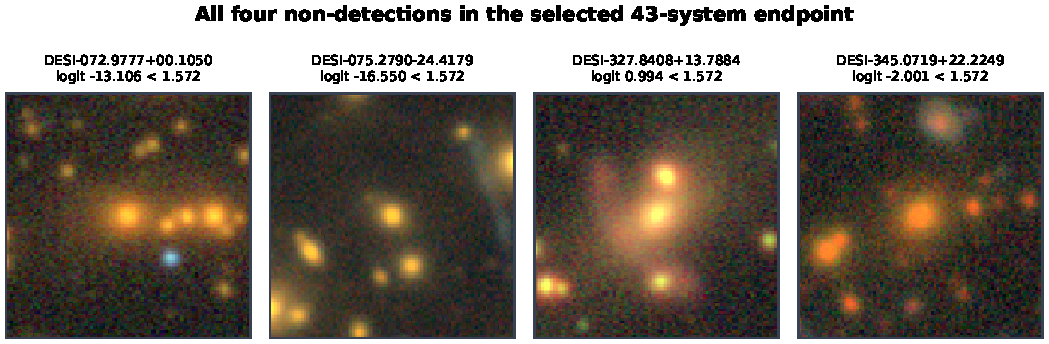
\includegraphics[width=0.82\textwidth]{figures/appendix_missed_selected_systems.pdf}
\end{center}
\refstepcounter{figure}\label{fig:missed_selected_systems}
\noindent\textbf{Figure~\thefigure.} All four non-detections among the 43
selected confirmed systems at
the primary threshold \(t_{10^{-3}}=1.5717214346\). Titles give the catalogue
name and native-float32 logit. Every panel uses the same complete
\(101\times101\)-pixel Legacy Survey \(z/r/g\) display mapping defined in
Equation~\ref{eq:rgb_preprocessing}; no panel-specific intensity rescaling or
crop is applied. The figure shows all four missed systems, not a
representative sample of the 43-system cohort.
\par\smallskip{\raggedright\noindent\textit{Alt text:} Four square Legacy Survey colour
cutouts arranged in one row. Each title identifies a confirmed system and
shows its logit below the common threshold. The images contain bright
foreground objects and surrounding structures with varied colour and
configuration.\par}
\medskip
\end{figure*}
\FloatBarrier

\subsection{Object-level provenance of the 43-system endpoint}

\label{app:confirmed_provenance}
The selected endpoint is not a uniformly dual-spectroscopic
sample. Table~\ref{tab:confirmed_43_provenance}
lists the object identifier, confirmation route, principal
object-level publication, and one representative recorded
foreground and source redshift for every evaluated system.
Multiple measurements and the complete evidence record are provided in
\texttt{confirmed\_43\_provenance.csv} in the reproducibility materials;
``--'' means that no
representative role-assigned redshift is recorded. The
confirmation-route column identifies whether displayed values
are secure, probable, low-confidence, or unverified.

\begin{table*}
\centering
\caption{Object-level provenance of the selected 43-system endpoint.}
\label{tab:confirmed_43_provenance}
{\scriptsize
\setlength{\tabcolsep}{3pt}
\renewcommand{\arraystretch}{0.92}
\begin{tabular}{p{0.14\textwidth}p{0.28\textwidth}p{0.24\textwidth}rr}
\toprule
Identifier & Confirmation route & Principal evidence & $z_{\rm foreground}$ & $z_{\rm source}$ \\
\midrule
\texttt{0361p000\_6437} & secure foreground and source spectra & \citep{Gladders2002,Gladders2003} & 0.773 & 4.8786 \\
\texttt{0442m235\_7484} & secure foreground and source spectra & \citep{Zitrin2011,Nakane2025} & 0.5049 & 1.09 \\
\texttt{0537m132\_1571} & secure foreground and source spectra & \citep{Lin2026} & 0.3866 & 2.30117 \\
\texttt{0572m102\_2469} & secure foreground and source spectra & \citep{Lin2026} & 0.74493 & 1.60376 \\
\texttt{0656m280\_3774} & secure foreground and source spectra & \citep{Lin2026} & 0.62107 & 1.17482 \\
\texttt{0728p000\_6851} & secure source; foreground spectrum unverified & \citep{Sand2005} & 0.430 & 2.007 \\
\texttt{0734m102\_4599} & secure foreground and source spectra & \citep{Richard2010,Lin2026} & 0.24820 & 1.043 \\
\texttt{0750m307\_2398} & secure foreground and source spectra & \citep{Lin2026} & 0.44137 & 1.44884 \\
\texttt{0753m245\_3999} & secure foreground and source spectra & \citep{Lin2026} & 0.32059 & 2.8290 \\
\texttt{0862m265\_8849} & secure foreground and source spectra & \citep{Lin2026} & 0.27534 & 2.17441 \\
\texttt{0870m362\_8874} & secure foreground and source spectra & \citep{Lin2026} & 0.3011 & 0.84611 \\
\texttt{0910m360\_2444} & secure foreground and source spectra & \citep{Lin2026} & 0.4883 & 1.43211 \\
\texttt{1219p105\_7293} & secure foreground and source spectra & \citep{Huang2026,Lin2026,Tran2022} & 0.475 & 1.23742 \\
\texttt{1409p185\_769} & secure foreground and source spectra & \citep{Huang2026,Tran2022} & 0.873 & 2.41673 \\
\texttt{1434p092\_2623} & secure lens; probable source spectrum & \citep{Tran2022} & 0.743 & 2.43243 \\
\texttt{1601p187\_3957} & secure foreground and source spectra & \citep{Lin2026,Tran2022} & 0.314 & 0.87872 \\
\texttt{1614m087\_3206} & secure lens; low-confidence source spectrum & \citep{Lin2026} & 0.82754 & 2.079 \\
\texttt{1655m060\_944} & secure foreground and source spectra & \citep{Zaborowski2023,Huang2026} & 0.4834 & 1.67511 \\
\texttt{1658p122\_150} & imaging/model; no secure dual spectra & \citep{Huang2026} & -- & -- \\
\texttt{1671p042\_499} & secure foreground and source spectra & \citep{Lin2026} & 0.35153 & 1.28023 \\
\texttt{1683p240\_1137} & secure foreground and source spectra & \citep{Kubo2009} & 0.3361 & 0.766 \\
\texttt{1686p167\_5461} & secure foreground and source spectra & \citep{Stark2013,Lin2026} & 0.537 & 1.718 \\
\texttt{1744p147\_5445} & secure foreground and source spectra & \citep{Lin2026} & 0.56486 & 2.41864 \\
\texttt{1894p150\_8726} & secure foreground and source spectra & \citep{Huang2026,Tran2022} & 0.57160 & 1.16149 \\
\texttt{1908p212\_1676} & secure foreground and source spectra & \citep{Lin2026} & 0.34832 & 1.48152 \\
\texttt{1928p017\_9908} & imaging/model; no secure dual spectra & \citep{Huang2026} & -- & -- \\
\texttt{1976p147\_245} & secure foreground and source spectra & \citep{Lin2026} & 0.26144 & 0.85834 \\
\texttt{2006p037\_9179} & secure foreground and source spectra & \citep{Lin2026,Tran2022} & 0.353 & 1.01590 \\
\texttt{2026p047\_4274} & secure foreground and source spectra & \citep{Huang2026,Lin2026,Tran2022} & 0.336 & 1.16757 \\
\texttt{2168m067\_3815} & secure foreground and source spectra & \citep{Zaborowski2023,Tran2022} & 0.26500 & 1.51409 \\
\texttt{2204p147\_3771} & secure foreground and source spectra & \citep{Stark2013,Pettini2010} & 0.741 & 1.433 \\
\texttt{2276p205\_1624} & imaging/model; no secure dual spectra & \citep{Huang2026} & -- & -- \\
\texttt{2349p167\_2044} & secure foreground and source spectra & \citep{Huang2026,Tran2022,Barone2026} & 0.409 & 1.833 \\
\texttt{2530p280\_351} & imaging/model; no secure dual spectra & \citep{Huang2026} & -- & -- \\
\texttt{2608p237\_3728} & secure foreground and source spectra & \citep{Lin2026} & 0.2296 & 0.97503 \\
\texttt{3108m062\_2639} & secure foreground and source spectra & \citep{Huang2026,Tran2022,Barone2026} & 0.79261 & 1.892 \\
\texttt{3277p137\_6699} & secure lens; probable source spectrum & \citep{Huang2026,Tran2022,Barone2026} & 0.20643 & 0.890 \\
\texttt{3409p280\_5325} & secure foreground and source spectra & \citep{Lin2026,Tran2022} & 0.343 & 0.96034 \\
\texttt{3418m020\_1357} & secure foreground and source spectra & \citep{Lin2026,Sand2005} & 0.330 & 2.237 \\
\texttt{3428m035\_4814} & secure foreground and source spectra & \citep{Lin2026} & 0.24592 & 1.05956 \\
\texttt{3431m042\_1867} & secure lens; low-confidence source spectrum & \citep{Lin2026} & 0.43519 & 0.58 \\
\texttt{3450p222\_3227} & secure foreground and source spectra & \citep{Wen2011,Stark2013} & 0.443 & 1.93 \\
\texttt{3459p235\_481} & secure foreground and source spectra & \citep{Lin2026} & 0.27653 & 1.29593 \\
\bottomrule
\end{tabular}
}
\end{table*}

\FloatBarrier

\subsection{Injection-target and matching support}

The 4,500 \(G_{\rm rec}\) targets are catalogue-selected injection targets, not
confirmed deflectors. Their Tractor types are 2,853 SER, 1,213 DEV, and 434
REX. Observed \(z\) magnitude has median 19.40, interquartile range
18.71--19.77, and range 13.29--20.00. The
selection manifest contains no homogeneous catalogue photo-\(z\) field for
these 4,500 rows. Photo-\(z\), velocity dispersion, stellar mass, and
environment therefore neither select these targets nor assign their SIE
parameters.

Under the score-blind assignment in Section~\ref{sec:decomposition_methods},
all 43 references receive unique targets. There are 168--4,229 admissible
targets per reference, and selected robust-IQR distances range from 0.108 to
1.140. Table~\ref{tab:gmatch_coverage} reports the measured support before
and after matching.

Direct checks of the stored bare and injected arrays verified their pairing
and the recorded target, source, lens, PSF, rendering, random, and flux
identities. No target-total flux floor, post-lensing flux rescaling, detector
score, or probe outcome enters matching or pair construction. The matching
set covers five measured image and catalogue quantities; homogeneous
deflector redshift, mass, environment, and observed-source brightness are
unavailable across all references.

\medskip
\noindent\begin{minipage}{\columnwidth}
\refstepcounter{table}\label{tab:gmatch_coverage}
\noindent\textbf{Table~\thetable.} Measured-covariate support for the 43
references, complete
\(G_{\rm rec}\) target roster, and 43 matched targets. Entries give
minimum/median/maximum; redshift, mass, environment, and source properties are
outside the matching set.
\begin{center}
\scriptsize
\resizebox{\columnwidth}{!}{%
\begin{tabular}{lrrr}
\toprule
Covariate & References & Target roster & Matched targets \\
\midrule
Observed \(z\) magnitude & 15.71/17.11/21.08 & 13.29/19.40/20.00 &
15.67/17.07/19.97 \\
S\'{e}rsic index & 1.00/4.34/6.00 & 0.50/2.60/6.00 &
0.66/4.27/6.00 \\
Axis ratio & 0.15/0.70/0.95 & 0.052/0.61/1.00 &
0.20/0.70/0.93 \\
\(r\)-band PSF FWHM (arcsec) & 1.01/1.27/1.81 & 0.98/1.39/1.72 &
1.00/1.27/1.70 \\
\(r\)-band depth (mag) & 24.10/24.47/25.75 & 23.79/24.30/26.44 &
24.10/24.41/25.65 \\
\bottomrule
\end{tabular}
}
\end{center}
\end{minipage}

\subsection{\(P_{\rm src}\) source construction and design}

For the regularised COSMOS F814W source construction defined in
Section~\ref{sec:source_models} \citep{Mandelbaum2012}, we report the realised
map-quality diagnostics and draw-count pilot below.

Of 81,499 catalogue rows, 770 satisfy the source criteria and 144 are
selected without detector outcomes for the final experiment. The maximum
structured--S\'{e}rsic centroid separation after construction is
\(7.34\times10^{-5}\) arcsec, the minimum retained positive-flux fractions
are 0.9010 and 0.9561 for the structured and S\'{e}rsic arms, respectively,
and their source-map pixel correlations range from 0.6190 to 0.9985
(median 0.9767). These diagnostics characterise construction fidelity; they
span visibly similar and dissimilar source-map pairs within the design.

A separate pilot used 1,584 pairs formed from 144 targets and 144 sources that
do not appear in the final experiment. Its joint distribution over the nine
target cells, eleven Einstein radii, and sixteen source strata is identical to
the final design. The pilot and final samples are disjoint in pair, underlying-scene,
target, spatial, physical, coordinate, pixel-hash, source, map-hash, and
ancestry fields. The number of photon draws was chosen before the final
experiment was scored.

The pilot scores 64 photon draws per pair. Table~\ref{tab:psrc_draw_pilot}
shows the empirical MCSE at each candidate count. The selection
rule chooses the smallest passing count, so eight draws are selected before
final scoring.

\medskip
\noindent\begin{minipage}{\columnwidth}
\refstepcounter{table}\label{tab:psrc_draw_pilot}
\noindent\textbf{Table~\thetable.} \(P_{\rm src}\) design-pilot photon-draw
selection. MCSE values and the target 0.01 are on the probability
scale; 0.01 equals one percentage point. Eight is the smallest
candidate count.
\begin{center}
\begin{tabular}{rrc}
\toprule
Draws & Measured MCSE & Pass \\
\midrule
8  & 0.000683 & Yes \\
16 & 0.000633 & Yes \\
32 & 0.000387 & Yes \\
64 & 0.000255 & Yes \\
\bottomrule
\end{tabular}
\end{center}
\end{minipage}


The final design contains 1,584 distinct targets in 1,219 spatial groups,
with the 99 target-cell--radius blocks and balanced source reuse specified in
Section~\ref{sec:paired_source_construction}.
Section~\ref{sec:paired_source_estimators} defines the corresponding weighting
and multiway uncertainty.

Before photon draws or detector scoring, all 1,584 paired expectation images
pass the convergence comparison at oversampling factors 4, 8, and
16. The maximum consecutive relative \(L_1\) difference is 0.002212, below
the 0.01 criterion. The eight selected photon draws then produce 12,672 pair-draw
rows per arm for the estimate reported in
Section~\ref{sec:paired_source_results}.

Under the reduced-cohort equal-cell rule, leave-one-source-out estimates range
from \(+0.524813\) to \(+0.580140\) percentage points, and
leave-one-spatial-group estimates range from \(+0.521104\) to \(+0.576299\)
points. No deletion changes the
sign. These are influence diagnostics rather than additional confidence
intervals.

\subsection{Noiseless known-source transfer}
\label{app:source_transfer_followup}

We tested the preparation route with 16 noiseless known-source cases covering
the retained source strata. Against an independently spatially refined
analytic reference, the maximum normalized \(L_1\) discrepancy is 0.08335 per
cent and the maximum production centroid residual is
\(3.72\times10^{-5}\) arcsec. All cases meet the global-\(L_1\),
centring, and normalization adequacy criteria, using limits of 1 per cent and
\(3\times10^{-4}\) arcsec for the first two quantities. Under the stricter
diagnostics, the local-pixel criterion is met in 1/16 cases and the shape
criterion in 0/16. The global and stricter summaries therefore characterize
different aspects of the same 16-case numerical check.

\subsection{Renderer reconciliation}
\label{app:renderer_reconciliation}

The renderer test contains 142 scenes: the 43 matched-design injections, the
order-48 scene, and one scene from each cell--radius stratum, with one overlap
among these groups. This sample tests numerical implementation across the
design but does not cover every production scene.
Every scene passes replay and production quadrature convergence,
independent optical-reference convergence after deterministic refinement
where required, comparison with an effective post-pixel Gaussian reference,
and comparison of production-support SIE deflections with an independent
implementation.
The effective-PSF comparison jointly changes operation order and FFT boundary
handling and therefore tests their combined implementation.

The maximum and 95th-percentile production/reference relative \(L_1\)
differences are 0.007695 and 0.005802. The maximum centroid difference is
0.02293 native pixel, the minimum pixel correlation is 0.999952, and the
maximum production-support SIE vector error is
\(9.06\times10^{-9}\) arcsec. These bounds summarize numerical agreement for
the audited scenes within the tested support.

The softened near-circular branch occurs in zero of the 49,500
realised \(G_{\rm rec}\) scenes and zero of the 1,584 \(P_{\rm src}\) pairs.
Production-support SIE tests pass; the separate boundary-specific test does
not meet its predefined criterion.

\vspace{-2pt}
\FloatBarrier
